%----------------------------------------------------------------------------------------
%	MANUALE D'USO
%----------------------------------------------------------------------------------------
\appendix
\section{Manuale d'uso}
Una volta avviato il sistema, all'utente viene presentata immediatamente la GUI del campo di gioco:
\begin{figure}[h]
	\centering
	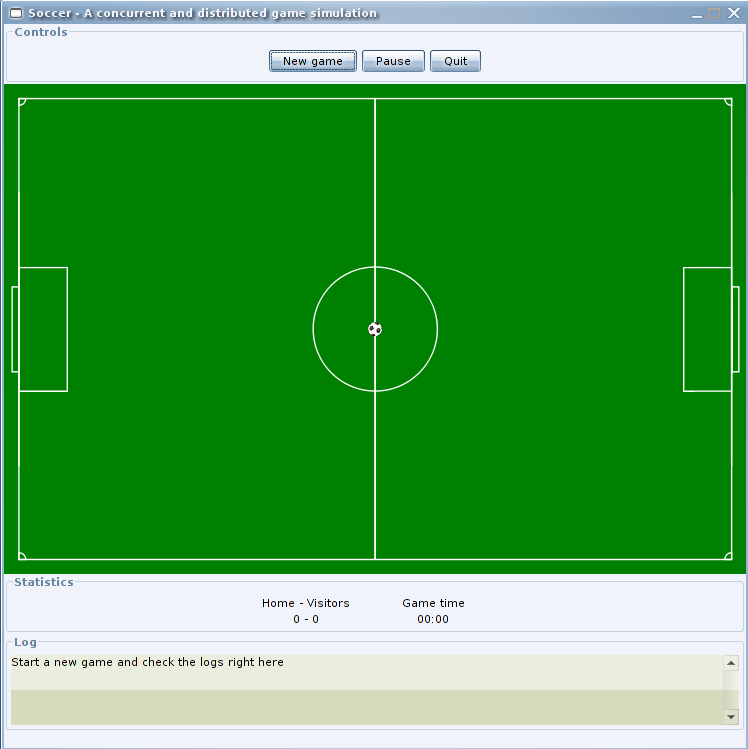
\includegraphics[scale=.5,width=\textwidth]{images/field_start}
	\caption{GUI del campo di gioco.}
\end{figure}

Sopra la rappresentazione del campo sono presenti i controlli per modificare lo stato del gioco, attraverso i quali è possibile iniziare una nuova partita, mettere in pausa quella corrente oppure terminarla. In basso, il pannello \emph{Statistics} riporta il risultato corrente della partita ed il tempo di gioco. Infine, è stato inserito un \emph{Log} in cui è possibile visualizzare gli eventi principali della partita in corso.\\

Per poter iniziare una nuova partita devono essere configurate entrambe le squadre partecipanti, tramite le interfacce dei manager. Per fare ciò, all'avvio del sistema, oltre alla GUI del campo di gioco, vengono presentate due semplici GUI (una per ogni squadra) da cui è possibile avviare i manager:
\begin{figure}[h]
	\centering
	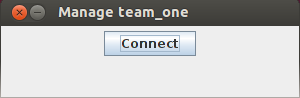
\includegraphics[scale=.5]{images/manager_connect}
	\caption{Finestra di avvio dei manager.}
\end{figure}

Premendo il pulsante \emph{Connect} viene di fatto avviato il manager, il quale si connette alla partita. Una volta premuto il pulsante \emph{New Game} presente nell'interfaccia del campo di gioco, viene presentata all'utente la GUI di configurazione della squadra:
\begin{figure}[h]
	\centering
	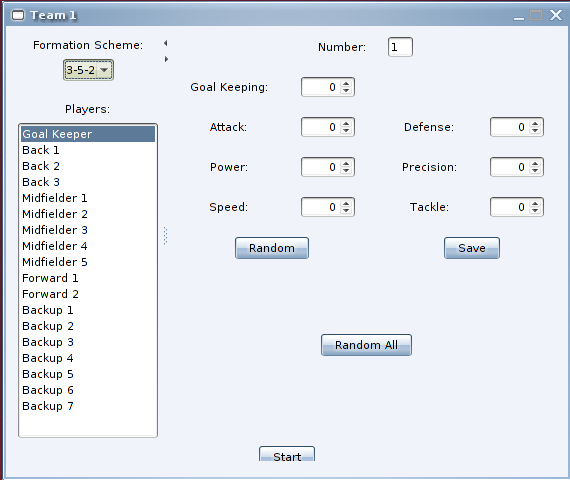
\includegraphics[scale=.5]{images/team_configuration}
	\caption{GUI di configurazione della squadra.}
\end{figure}

L'interfaccia è suddivisa in due parti: il pannello laterale e il pannello delle statistiche. Il pannello laterale permette di cambiare la formazione della squadra utilizzando il menù a tendina, intitolato \emph{Formation Scheme} e posizionato in alto; inoltre permette di selezionare comodamente ciascun giocatore dalla lista \emph{Players}. Dopo aver selezionato un giocatore, è possibile vedere e modificare le sue statistiche dal pannello di destra. All'avvio, tutte le statistiche dei giocatori assumono valore zero. Dal pannello delle statistiche è possibile impostare manualmente il numero di maglia del giocatore e tutte le sue statistiche. Quest'ultime devono essere comprese tra zero e cento. Il pulsante \emph{Random} permette di generare casualmente tutte le statistiche del giocatore correntemente selezionato. Una volta assegnati i valori desiderati alle statistiche, le modifiche effettuate vanno salvate tramite il pulsante \emph{Save}. \`{E} anche possibile generare casualmente e salvare tutte le statistiche di tutti i giocatori utilizzando il pulsante \emph{Random All}. Infine, premere \emph{Start} per terminare la configurazione della squadra.\\

Una volta terminata la configurazione di entrambe le squadre, la partita ha inizio e i giocatori iniziano ad entrare in campo. Ecco lo stato dell'interfaccia del campo di gioco una volta configurate le squadre e avviata la partita:
\begin{figure}[h]
	\centering
	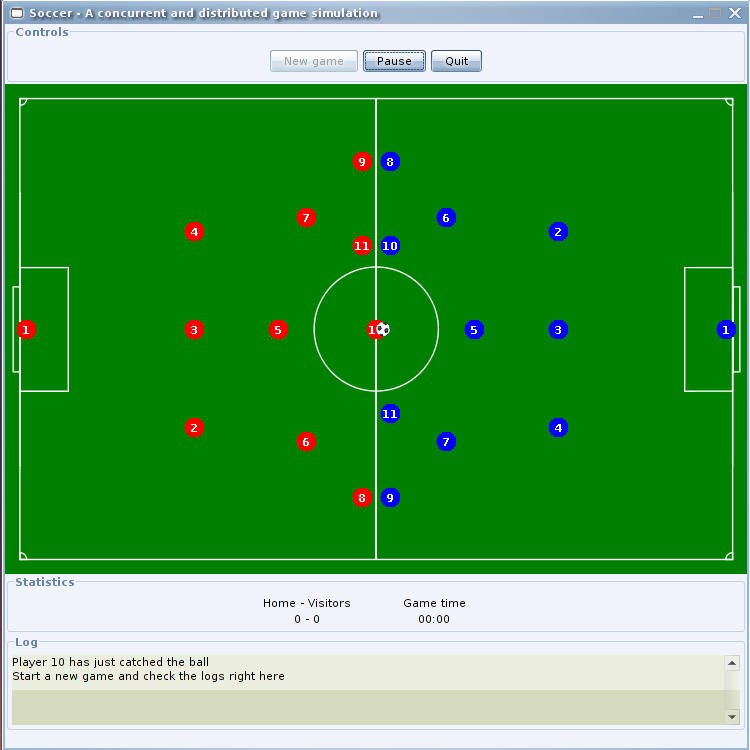
\includegraphics[scale=.5,width=\textwidth]{images/field}
	\caption{GUI del campo di gioco a partita avviata.}
\end{figure}
\newpage
Durante il corso della partita ciascun manager ha a disposizione una GUI dalla quale può gestire la propria squadra:
\begin{figure}[h]
	\centering
	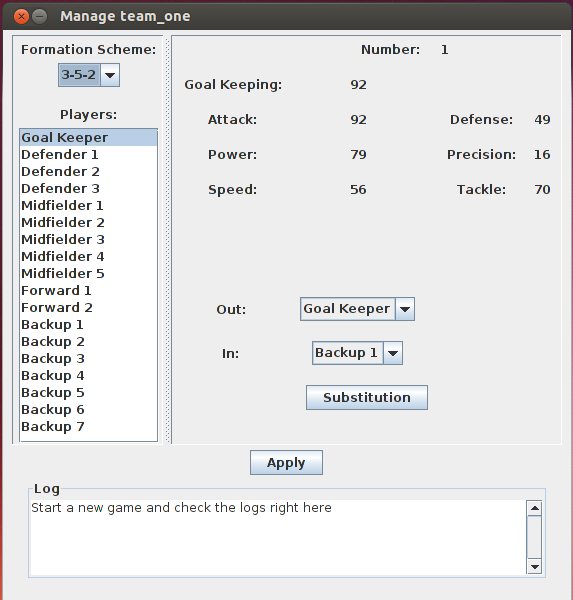
\includegraphics[scale=.5]{images/team_manager}
	\caption{GUI del manager.}
\end{figure}

Sulla sinistra, si può vedere lo stesso pannello laterale presente nella finestra di configurazione delle squadre: da esso è possibile cambiare la formazione della squadra e selezionare un giocatore. 

Il pannello di destra riporta le statistiche del giocatore selezionato. Si noti che non è possibile modificare le statistiche dei giocatori a partita avviata. In questo pannello sono presenti anche i comandi per avviare una sostituzione. In questo contesto, il menù a tendina \emph{Out} permette di selezionare il giocatore da sostituire, mentre il menù a tendina \emph{In} permette di selezionare il giocatore da far entrare in campo. Per confermare la sostituzione è sufficiente premere \emph{Substitution}. \`{E} possibile effettuare una sostituzione per volta.

Per salvare e applicare le modifiche effettuate, siano esse una cambio di formazione o una sostituzione, premere il pulsante \emph{Apply}. 

Infine, in basso, è presente un \emph{Log} da cui è possibile visualizzare comodamente gli eventi principali della partita in corso.